\chapter{Approach}\label{approach}

\section{Overview}\label{sec:overview}
\TODO{overview}

\section{Experimental Setup}\label{sec:experimental_setup}
This section details the experimental setup used to investigate the hypotheses outlined in Section~\ref{sec:research_questions}, including data formatting techniques, model configuration, training procedures, and evaluation metrics employed in the experiments. The experiments cover analysis of the effects of positional encodings, data formatting, and inclusion of sub-task data on the length generalization capabilities of transformer models in the multi-digit integer addition task.

\subsection{Data Formatting}\label{subsec:data_formatting}
Various data formatting techniques are employed and their effects on model generalization is exampined. All experiments use character-level tokenization; every character (digit, letter, symbol such as ``\texttt{+}'', ``\texttt{=}'', or space) is treated as an individual token. The vocabulary consists of 100 printable ASCII characters, ensuring that each token is represented uniquely. While character tokenization as such is a simple and flexible method, it is worth noting that current state-of-the-art LLMs use other subword tokenization schemes such as Byte-Pair Encoding (BPE) \parencite{sennrich_neural_2016,brown_language_2020}. Table~\ref{tab:data_formatting_examples} summarizes the different data formatting techniques with examples.

\paragraph{Standard Format}
In the standard format, input sequences are represented as ``\verb|$a+b=c$|'', where $a$ and $b$ are the operands, and $c$ is the sum. The dollar signs ``\verb|$|'' denote the start and end of the sequence; the final ``\verb|$|'' also serves as the end-of-sequence token during autoregressive generation, stopping the process once it is generated. The plus ``\verb|+|'' and equals ``\verb|=|'' symbols separate the operands and the answer, respectively. For example, adding 123 and 456 is formatted as:
\begin{center}
    \verb|$123+456=579$|
\end{center}
This format serves as the baseline, with other formatting methods building upon it.

\paragraph{Zero Padding}
Zero padding involves aligning the digits by prepending operands and answers with leading zeros to match a fixed length $N_\text{pad}$. For instance, if $N_\text{pad}=5$, the addition of 123 and 456 becomes:
\begin{center}
    \verb|$00123+00456=00579$|
\end{center}
This method ensures that corresponding digits in different numbers always occupy the same absolute positions in the sequence, simplifying the learning of positional relationships. However, it does not actually solve the problem, since it requires prior knowledge of the maximum sequence length and can't be applied to sequences longer than $N_\text{pad}$.

\paragraph{Reversing}
Reversing the digits of operands and/or the answer switches the digit ordering to start with least significant digits, which follows the flow of operations like carry propogation. For example, reversing the operands yields:
\begin{center}
    \verb|$321+654=579$|
\end{center}
Reversing both operands and the answer gives:
\begin{center}
    \verb|$321+654=975$|
\end{center}
Reversing the operands alone, in principle, should not significantly impact performance, as the model can learn appropriate attention patterns to handle reversed sequences. However, reversing the answer theoretically simplifies the task by localizing carry propagation - since the model generates the output from left to right and can compute each digit independently instead of being forced to implicitly perform the carry propagation through the complete answer before generating the first answer digit.

\paragraph{Random Spaces}
Random spaces are inserted between symbols in the input sequence to disrupt fixed positional patterns and encourage the model to learn position-invariant representations. The number of spaces inserted is controlled by a parameter $\rho$, representing the maximum ratio of random spaces to non-space tokens in the operands. The maximum number of random spaces is calculated as $n_{\text{max}} = \rho \times L$, where $L$ is the length of the sequence (excluding the start token \texttt{\$}). The actual number of spaces $n$ is sampled uniformly from the set $\{0, \dots, n_{\text{max}}\}$. For example, if $\rho = 0.5$ and $L = 10$, then $n_{\text{max}} = 5$, and $n$ is randomly chosen from $\{0, 1, 2, 3, 4, 5\}$. The spaces are inserted at random positions within the operands. In all presented experiments, $\rho = 0.5$ when random spaces are enabled. An example of an input sequence with random spaces is:
\begin{center}
    \verb|$1 23 +4  5 6=579$|
\end{center}

\paragraph{Scratchpad}
A scratchpad, or chain-of-thought, includes intermediate computational steps before the final answer, promoting step-by-step reasoning. This format also allows for the evaluation of intermediate results and aids in understanding the model's reasoning process. However, it requires task-specific data and therefore is not a general method. The scratchpad consists of reversed operands, modular addition with carry notation separated by semicolons, and the final answer separated by a vertical bar. An example with comments describing the parts is given below (the line breaks are included for convenience and not part of the actual sequence):
\begin{center}
    \begin{tabular}{l l}
        \verb|$567+789=7 6 5 + 9 8 7;| & \textit{Input equation and reversed operands}             \\
        \verb|c=0,7+0+0=7,c=0;|        & \textit{Sum of units digit, no carry initially}           \\
        \verb|6+9+0=5,c=1;|            & \textit{Sum of tens digit, carry generated}               \\
        \verb|5+8+1=4,c=1;|            & \textit{Sum of hundreds digit and carry, carry generated} \\
        \verb|0+7+1=8,c=0|             & \textit{Sum of thousands digit and previous carry}        \\
        \texttt{|8457\$}               & \textit{Final result}
    \end{tabular}
\end{center}

This sequence represents the addition of 567 and 789 with detailed computation steps, where \texttt{c} denotes the carry variable.


\begin{table}[ht]
    \centering
    \caption{Examples of Data Formatting Techniques}
    \label{tab:data_formatting_examples}
    \begin{tabular}{ll}
        \toprule
        \textbf{Format}                                        & \textbf{Example}                                           \\
        \midrule
        Plain                                                  & \verb|$123+456=579$|                                       \\
        Zero Padding (to length 5)                             & \verb|$00123+00456=00579$|                                 \\
        Reversed Operands                                      & \verb|$321+654=579$|                                       \\
        Reversed Answer                                        & \verb|$123+456=975$|                                       \\
        Reversed Operands and Answer                           & \verb|$321+654=975$|                                       \\
        Random Spaces                                          & \verb|$12  3 +45 6=579$|                                   \\
        Scratchpad                                             & \begin{tabular}[t]{@{}l@{}} \verb|$567+789=7 6 5 + 9 8 7;| \\
                                                                     \verb|c=0,7+0+0=7,c=0;|                     \\
                                                                     \verb|6+9+0=5,c=1;|                         \\
                                                                     \verb|5+8+1=4,c=1;|                         \\
                                                                     \verb|0+7+1=8,c=0|                          \\
                                                                     \texttt{|8457\$}
                                                                 \end{tabular} \\
        Subtask Prefix (placeholder \texttt{xxx})\footnotemark & \verb|xxx$123+456=321+654$|                                \\
        \bottomrule
    \end{tabular}
\end{table}

\footnotetext{See Section~\ref{subsec:data_gen} for details on subtasks and corresponding prefixes.}


\subsection{Data Generation}\label{subsec:data_gen}

The training and test datasets for the experiments are systematically generated to evaluate the length generalization capabilities of transformer models on integer addition tasks. Each dataset consists of addition problems where both operands \( a \) and \( b \) are positive integers of equal number of digits, denoted as the \emph{digit length}. An addition problem involving operands of \( n \) digits is referred to as an \( n \)-digit or \( n \times n \) addition problem. For instance, a ``4-digit'' or ``4x4'' addition refers to both operands having exactly four digits.

Multiple datasets are created, each encompassing a specific range of in-distribution (ID) digit lengths for training and corresponding out-of-distribution (OOD) digit lengths for testing. The datasets are designed to assess the models' ability to generalize to sequence lengths beyond those seen during training. In each case, the datasets are split into training, validation, and test sets. The training set contains a specified number of ID digit length samples, while separate validation and test datasets are generated for ID and OOD digit lengths. To prevent data contamination, all samples in the validation and test sets are unique and not present in the training set.

The operand values are randomly sampled to ensure uniform coverage of possible combinations within the specified digit lengths. Numbers are generated such that they have exactly the specified number of digits (i.e., they do not start with zero). Unless specified otherwise, no attempt is made to balance the digit distribution nor the number of carries required in the addition operations across the samples.

Following the methodology of \cite{lee_teaching_2023}, for 1-digit operands (1x1 addition), all possible 100 combinations (operands ranging from 0 to 9) are included in the training dataset and therefore excluded from the test sets to avoid overlap. For 2-digit operands, 900 samples are randomly selected, and for 3-digit operands, 9000 samples are used. For digit lengths of 4 and above, an equal number of samples per digit length are randomly generated to fill the remaining training set size.

Out-of-distribution test sets are constructed by including digit lengths not present in the training data. Each OOD test set contains 1000 unique samples for each OOD digit length to evaluate the model's length generalization performance.

\paragraph{Sub-Task Data}

To enhance the compositional learning abilities of the models and investigate their impact on length generalization, various sub-task data was incorporated into some datasets. The sub-tasks include \emph{reversing}, \emph{carry detection}, \emph{digit-wise modular addition}, and \emph{digit alignment}. Each sub-task focuses on a specific aspect of the addition process, aiming to help the model learn underlying algorithmic components that could facilitate better generalization.

In contrast to the scratchpad approach, where intermediate computations are appended sequentially (leading to potential compounding errors), the sub-task training treats each sub-task as an independent auxiliary task. This method allows the model to learn each sub-task simultaneously without relying on the outputs of other tasks. Conversely, sub-task training implicitly involves composing multiple algorithmic parts due to pressure from the complete addition problem included alongside sub-tasks, instead of enforcing composition in each sequence.

To allow the model to differentiate between the sub-tasks each example includes a 3-letter task prefix, resulting in the format \texttt{xxx\$a+b=c\$}, where \texttt{xxx} denotes the sub-task identifier, and \texttt{c} represents the sub-task-specific output.

The sub-tasks, their prefixes, and their formats are as follows:

\begin{itemize}
    \item \textbf{Digit Alignment} (\texttt{ali}): Focuses on aligning the digits of the two operands for position-wise operations. The model learns to output the corresponding digit pairs from each operand.

          Example: \texttt{ali\$1234+4567=1+4,2+5,3+6,4+7\$}

    \item \textbf{Reversing} (\texttt{rev}): Involves reversing the digits of each operand. This sub-task helps the model understand the reversal operation, which inverts the propagation order from least significant digit to most.

          Example: \texttt{rev\$1234+4567=4321+7654\$}

    \item \textbf{Carry Detection} (\texttt{car}): Requires the model to identify positions where a carry operation would occur during addition. This sub-task is essentially a lookup operation from 2 digits to a binary value. The output is a string of ``c''s and dashes, indicating positions with and without carries respectively.

          Example: \texttt{car\$1234+4567=---c\$}

    \item \textbf{Digit-wise Modular Addition} (\texttt{mad}): The model performs addition modulo 10 on each pair of corresponding digits without considering carries. This sub-task is also in principle a lookup operation, from 2 digits to another digit.

          Example: \texttt{mad\$1234+4567=5791\$}

    \item \textbf{Addition} (\texttt{add}): The standard addition task, where the model computes the sum of the two operands. This serves as the main task and is included alongside sub-tasks in the dataset to facilitate composition of their output.

          Example: \texttt{add\$1234+4567=5801\$}
\end{itemize}

\paragraph{Datasets}

Several datasets were generated to support different experiments, each tailored to investigate specific aspects of length generalization and compositional learning. Below, we detail each dataset and its composition:

\begin{itemize}
    \item \texttt{1-3\_digit}:
          \begin{itemize}
              \item \textbf{Training Set}: Contains 10,000 samples of addition problems where the operands have 1 and 3 digits. The dataset follows the methodology of \cite{lee_teaching_2023} and is used to replicate their baseline results.
              \item \textbf{Test Sets}: Separate test sets are created for each digit length from 1 to 4 digits, including OOD lengths of 2- and 4-digit addition problems not seen during training.
          \end{itemize}

    \item \texttt{1-7\_digit}:
          \begin{itemize}
              \item \textbf{Training Set}: Includes addition problems with operands ranging from 1 to 7 digits.
              \item \textbf{Test Sets}: Comprises test samples for digit lengths 1 to 8, with 8-digit addition serving as the OOD evaluation.
              \item \textbf{Purpose}: Replicates the extended baseline from \cite{lee_teaching_2023}, examining generalization to slightly longer sequences.
          \end{itemize}

    \item \texttt{generalize\_to\_longer}:
          \begin{itemize}
              \item \textbf{Training Set}: Consists of 1 million samples with digit lengths from 1 to 17 and 19 digits, intentionally excluding 18-digit problems to create an interpolation gap.
              \item \textbf{Test Sets}: Includes OOD test sets for 18-digit (interpolation) and 20-digit (extrapolation) addition problems.
              \item \textbf{Purpose}: Evaluates the model's ability to generalize to unseen lengths within (interpolation) and beyond (extrapolation) the training range.
          \end{itemize}

    \item \texttt{generalize\_to\_longer\_mini}:
          \begin{itemize}
              \item \textbf{Training Set}: Contains addition problems with digit lengths of 1 to 7 digits and 9 digits, deliberately omitting 8-digit problems.
              \item \textbf{Test Sets}: OOD test sets for 8-, 10-, and 11-digit addition problems.
              \item \textbf{Scales}: Training data is generated at multiple scales, with datasets of 10K, 100K, 1M, and 10M examples to study the impact of dataset size, where ``K'' denotes thousands and ``M'' denotes millions.
              \item \textbf{Purpose}: Investigates length generalization across different data scales and the effect of missing intermediate digit lengths.
          \end{itemize}

    \item \texttt{generalize\_to\_longer\_mini\_multitask}:
          \begin{itemize}
              \item \textbf{Composition}: Similar to \texttt{generalize\_to\_longer\_mini}, but includes all five sub-tasks (addition, reversing, carry detection, digit-wise modular addition, digit alignment) in the training data. Contains 2 variants for each scale: addition-only and multi-task training (including sub-tasks).
              \item \textbf{Scales}: Generated at the same data scales as above.
              \item \textbf{Purpose}: Examines the effect of sub-task training on compositionality and length generalization as compared to addition-only training.
          \end{itemize}

    \item \texttt{generalize\_to\_longer\_mini\_gap}:
          \begin{itemize}
              \item \textbf{Training Set}: Comprises 100K addition problems with digit lengths of 1 to 7 digits and 11 digits, creating a larger ``gap'' in the training digit lengths.
              \item \textbf{Test Sets}: OOD test sets for digit lengths 8, 9, 10 (interpolation), and 12, 13 (extrapolation).
              \item \textbf{Purpose}: Designed to evaluate whether the model can generalize across a larger gap in sequence lengths.
          \end{itemize}
\end{itemize}

\subsection{Model Configuration}

Transformer decoder models are used as described in the Background chapter (Section~\ref{subsec:types_transformers}). Unless specified otherwise, a standard transformer decoder architecture is employed. The models are varied along several dimensions to assess their impact on performance:

\begin{itemize}
    \item \textbf{Number of layers (depth)}: The number of decoder layers.
    \item \textbf{Model dimension (width)}: The dimensionality of the model embeddings and hidden representations.
    \item \textbf{Number of attention heads}: The number of attention heads $h$ is chosen such that $d$ is divisible by $h$, commonly set to powers of 2.
    \item \textbf{Feed-forward layer dimension}: The hidden dimension of the feed-forward layers is set to $d_{\text{ff}} = 4 \times d$.
    \item \textbf{Context length}: The maximum input sequence length, denoted as $L_{\text{max}}$, is set based on the task requirements and is only relevant for models with absolute positional encodings.
\end{itemize}

Unless otherwise noted, models use absolute positional encodings. For experiments involving different positional encoding schemes, the specific configurations are detailed in the respective sections.

\subsection{Training and Evaluation}

\paragraph{Training Setup}
Overall, the training parameters from the NanoGPT \parencite{karpathy_nanogpt_2022} are used with modified number of steps, learning rates, and batch sizes. All models are trained using the AdamW optimizer with hyperparameters as follows (see Table~\ref{tab:optimizer_hyperparameters}):

\begin{table}[h]
    \centering
    \caption{Optimizer Hyperparameters}
    \label{tab:optimizer_hyperparameters}
    \begin{tabular}{lcc}
        \toprule
        Hyperparameter & Value              \\
        \midrule
        Optimizer      & AdamW              \\
        Learning rate  & $3 \times 10^{-4}$ \\
        Betas          & $(0.9, 0.999)$     \\
        Epsilon        & $1 \times 10^{-8}$ \\
        Weight decay   & $0.1$              \\
        \bottomrule
    \end{tabular}
\end{table}

A learning rate scheduler with linear warm-up and cosine decay is used; for the first $T_{\text{w}} = 100$ iterations, the learning rate increases linearly from $0$ to the chosen learning rate. After warm-up, the learning rate at the current iteration $\eta(t)$ is cosine-annealed to a minimum learning rate of $\eta_{\text{min}} = 0.1 \times \eta$ over the course of training until maximum number of iteartions $T_{\text{max}}$ according to the formula:
\[
    \eta(t) =
    \begin{cases}
        \eta_{\text{max}} \times \dfrac{t}{T_{\text{w}}},                                                                                                                          & \text{if } t < T_{\text{w}}                        \\
        \eta_{\text{min}} + \dfrac{1}{2} (\eta_{\text{max}} - \eta_{\text{min}}) \left[1 + \cos\left( \pi \dfrac{t - T_{\text{w}}}{T_{\text{max}} - T_{\text{w}}} \right) \right], & \text{if } T_{\text{w}} \leq t \leq T_{\text{max}} \\
        \eta_{\text{min}},                                                                                                                                                         & \text{if } t > T_{\text{max}}
    \end{cases}
\]
where $t$ is the current iteration.

The batch size is selected based on the task, the model size and the sequence length to maximize GPU utilization while avoiding memory constraints. For large models or long sequences, gradient accumulation over multiple steps is employed to achieve an effective batch size. The number of training epochs is not set explicitly, rather the number of optimizer steps (iterations) is used. Answer loss masking (as described in Section~\ref{subsec:training_inference}) is applied during training unless specified otherwise. This means that the loss is computed only over the tokens corresponding to the answer part of the sequence, excluding any start tokens or padding tokens.

\paragraph{Inference Procedure}
During inference, top-$k$ sampling with $k=1$ is used, which corresponds to greedy decoding by selecting the token with the highest probability at each timestep. Although beam search was implemented and tested, it did not yield significant improvements due to the sharpness of the output distribution; the model's predictions are typically highly confident, with the softmax probabilities concentrated on a single token.

\paragraph{Evaluation Metrics}
For all experiments, the models are evaluated using two primary metrics:

\begin{itemize}
    \item \textbf{Cross-Entropy Loss}: Calculated over the answer tokens only, providing a measure of the model's average log-likelihood of the correct answer tokens. Lower loss values indicate better performance. The loss is also related to the \emph{perplexity} of the model, which is the exponential of the loss and is often used as a metric in language modeling tasks. The perplexity represents the average number of choices the model has for the next token, with lower values indicating better performance.
    \item \textbf{Accuracy}: Defined as the proportion of samples where all answer tokens are predicted correctly, also known as full match accuracy. A single incorrect digit in the answer results in the sample being marked as incorrect. To compute the accuracy, autoregressive inference (as described in Section~\ref{subsec:training_inference}) is used to generate the full answer sequence one token at a time until the end-of-sequence token is predicted or the maximum sequence length is reached. Higher accuracy values indicate better performance. The cross-entropy loss can be used to compare model performance when the accuracy is the same, e.g. when models have been trained short of full convergence and task accuracy is 0.
\end{itemize}

During training, both training and validation losses are recorded to monitor the learning dynamics. Models are evaluated on validation sets corresponding to both in-distribution (ID) and out-of-distribution (OOD) digit lengths to assess their generalization capabilities.


\section{Limitations of Absolute Positional Encodings}\label{sec:absolute_positional_limitations}
Assess the limitations of absolute positional encodings in enabling length generalization for integer addition tasks.

summarize findings: by itself, absolute pos encoding is unable to generalize even to slightly longer sequences, and fails to interpolate or extrapolate to unseen lengths. Seems to be due to inability to continue attention patterns beyond training lengths (evidence: attention maps, where unlike absolute PE, abacus has crisp attn maps because it can precisely select correct digits based on position, abs with addition of random spaces smoothes attn maps, which helps it generalize a tiny bit). Also, next token entropy analysis shows that models trained on 1-7 and 9 digits are very confident in their predictions for in-distribution lengths, but become increasingly uncertain for OOD lengths, especially for longer sequences, trying to end the sequence and token distribution becomes smoother, prob of correct token goes to 0. So, aligning the correct digits is the main issue, consistent with literature that vanilla transformer struggles to perform index-addressing operations.
If we fix the digit alignment part for the model (e.g. abacus embeddings) and don't change anything else, models can generalize to longer sequences well. But, how can we push absolute vanilla setup, without special embeddings, to generalize to longer sequences? -> random spaces added to sequence can help weakly generalize: generalizing to interpolating lengths and 1 digit longer sequences. In next section, effects of different data formatting (including random spaces) on length generalization are explored.

\TODO{refer to string algo tasks in appendix that isolate indexing issues}

\subsection{Length Generalization Baseline}
Establish the baseline performance of models with absolute positional encodings on length generalization. The first subplot in figure in TODO will show how: when trained on 1 and 3 digits, the model fails 2 and 4 digits, and when trained on 1-7 digits, the model fails 8 digits.

Describe how models are trained on addition tasks with operands of certain digit lengths and tested on both seen and longer unseen digit lengths. Highlight the expectation that models will struggle with sequences longer than those seen during training, supporting the hypothesis that absolute positional encodings limit generalization. In this case, there is no generalization, neither in interpolation nor extrapolation OOD lengths.

\paragraph{Longer Training Sequences}
want to test whether training on longer sequences changes this. The 2nd subplot referenced in figure placeholder shows where even training on 1-17 and 19 digit additions does not enable generalization to 18 and 20 digit additions in vanilla.

\TODO{PLOT 3x3 and 7x7 experiments, as well as 1-17 and 19 digit train, 18 and 20 OOD failures}
\label{fig:baseline_and_longer}


\paragraph{Next Token Uncertainty Analysis}

\TODO{PLOT average plots for entropy for next token prediction distributions, probabilities of correct and EOS tokens over generated answe sequence. Given a model trained on 1-7 and 9 digit lengths, look at cases: in-dist lengths (everything fine), , and OOD lengths see how it goes nuts}
\label{fig:next_token_entropy}

\subsection{Digit Alignment-focused PE Improves Generalization}
hypothesis: digit alignment is the root issue. Train models with absolute, absolute + random spaces, and abacus models in same setup (100k samples, 1-7 training, 8 and 10 OOD testing). Look at attention maps to see patterns, and look at mistakes (where they happen).

\TODO{PLOT abacus vs abs results}
\label{fig:digit_align_pe}

\TODO{PLOT attn maps from above models, discuss differences}
\label{fig:digit_align_attn_maps}


\subsection{Breaking Positional Patterns in Absolute PE Allows Weak Generalization}
Investigate the impact of introducing random spaces into input sequences on length generalization. The hypothesis is that random spaces disrupt fixed positional patterns that the model might overfit to, encouraging it to learn more robust representations. It does help a bit.

\TODO{PLOT results for abs + randspaces vs abs without}

\TODO{PLOT abs + randspaces vs abs without attn maps}
\label{fig:rand_spaces_attn_maps}


\section{Impact of Data Formatting on Length Generalization}\label{sec:data_formatting_improvement}
Investigate how different data formatting strategies impact the model's ability to generalize to longer sequences. Reversing vs not reversing the answer/operands, random spaces (important), scratchpad, zero padding.

\TODO{summarize findings}

\subsection{Zero Padding}
Assess how zero-padding operands to a fixed length influences generalization performance.

Note: Findings from Experiments 7-9 (included in the Appendix) are summarized here. These experiments explore zero-padding but are not central to the main hypotheses.

Highlight that while zero padding aligns digits and may improve performance on sequences up to the maximum padded length, it may not facilitate generalization to longer sequences without prior knowledge of maximum lengths.

\TODO{plot zero padded exp 7x7 I think - need to check}

\subsection{Reversing}
Examine the impact of reversing operands and the answer on model generalization. Theoretically, reversing operands should not matter and reversing answer should help. But, for Abacus pos encoding operands should be reversed. Reversing the answer theoretically makes the task simpler, and experimentally results in step-wise loss jumps. Interestingly, in both cases (whether answer reversed or not) i find that models start correctly predicting most significant digits, and over the training predict more and more digits right until the max in-distribution length. This happens even if answers are reversed, where model predicts incorrect then correct digits.

\TODO{PLOT abspe revans vs norev 128-dim, 4-layer from exp 30}

\subsection{Random Spaces}
Examine the effect of introducing random spaces into input sequences on length generalization.

Note: Experiment 23 focuses on this aspect. It trains models on 1-7 and 9-digit additions with random spaces added to the input sequences and tests on 8 and 10-13 digits.

Discuss the hypothesis that adding randomness in spacing disrupts positional patterns that the model might overfit to, thereby encouraging it to learn more robust representations.

\paragraph{Interpolating OOD Digit Lengths}
Now, question is whether a larger gap of interpolation OOD lengths can also be closed. Discuss experiment where there is a larger gap in in-distribution lengths: trained on 1-7 and 11 digits, tested on OOD 8, 9, 10, and 12, 13 digits.

\TODO{PLOT larger gap experiment (abs and abs + random spaces), can also be closed with random spaces}
\label{fig:larger_gap}


\subsection{Scratchpad}
Scratchpad by itself does not help generalization, but helps mistake analysis. Random spaces also work in the scratchpad setup. So overall, scratchpad is not practical for other tasks (need correct intermediate computations, not always available nor known in practice), but can help understand mistakes in intermediate tasks. In literature, scratchpad was shown to help large models generalize, so it seems that smaller models can't leverage it as much.
\TODO{discuss results from scratchpad in text, accuracy and loss numbers}

\TODO{PLOT scratchpad evaluation results (violin plots of intermediate task accuracies, etc)}
\label{fig:scratchpad_eval}


\section{Sub-task Learning for Compositionality}\label{sec:subtask_learning}
Explore the hypothesis that incorporating sub-task data can improve the model's compositionality and length generalization capabilities by helping learn the underlying algorithmic components of the task.
Experiment is a comprehensive analysis of sub-task learning across model dimensions (width) ranging from 64 to 1536 and dataset sizes 10K, 100K, 1M, 10M examples, each in addition-only and multi-task training settings. The main idea is that mix task training sometimes improves OOD loss, effect is especially pronounced for smaller models and smaller dataset sizes.

\TODO{summarize findings}


\subsection{Sub-Tasks Marginally Improve Length Generalization}
Analyze addition-only vs sub-task (mix) training across model dimensions and dataset sizes. Also look at plots of OOD val-loss vs ID val-loss, see if it helps overfitting. Refer to Figure \ref{fig:exp_27_val_loss_vs_n_embd}. Interesting point to be made, how smaller models (64 dimensions and 8 heads means 8 dimensions per head, that is low compared to usually used models in literature for these tasks) benefit more (unintuitive). Now it is not explored why this is, but tentative hypothesis might be that large models overfit to the tasks, and have the capacity to overfit to multi-task as well and see no benefit (i.e. they just memorize the data, and since in mix the train data size is same as add-only, they can memorize it as well). But smaller models are even more forced to learn a generalizing algorithm, where subtasks help.

\TODO{TABLE of results (also show difference between add-only and mix task training)}
\label{tab:subtask_results}


\TODO{PLOT replot val loss vs embd}
\begin{figure}[h!]
    \centering
    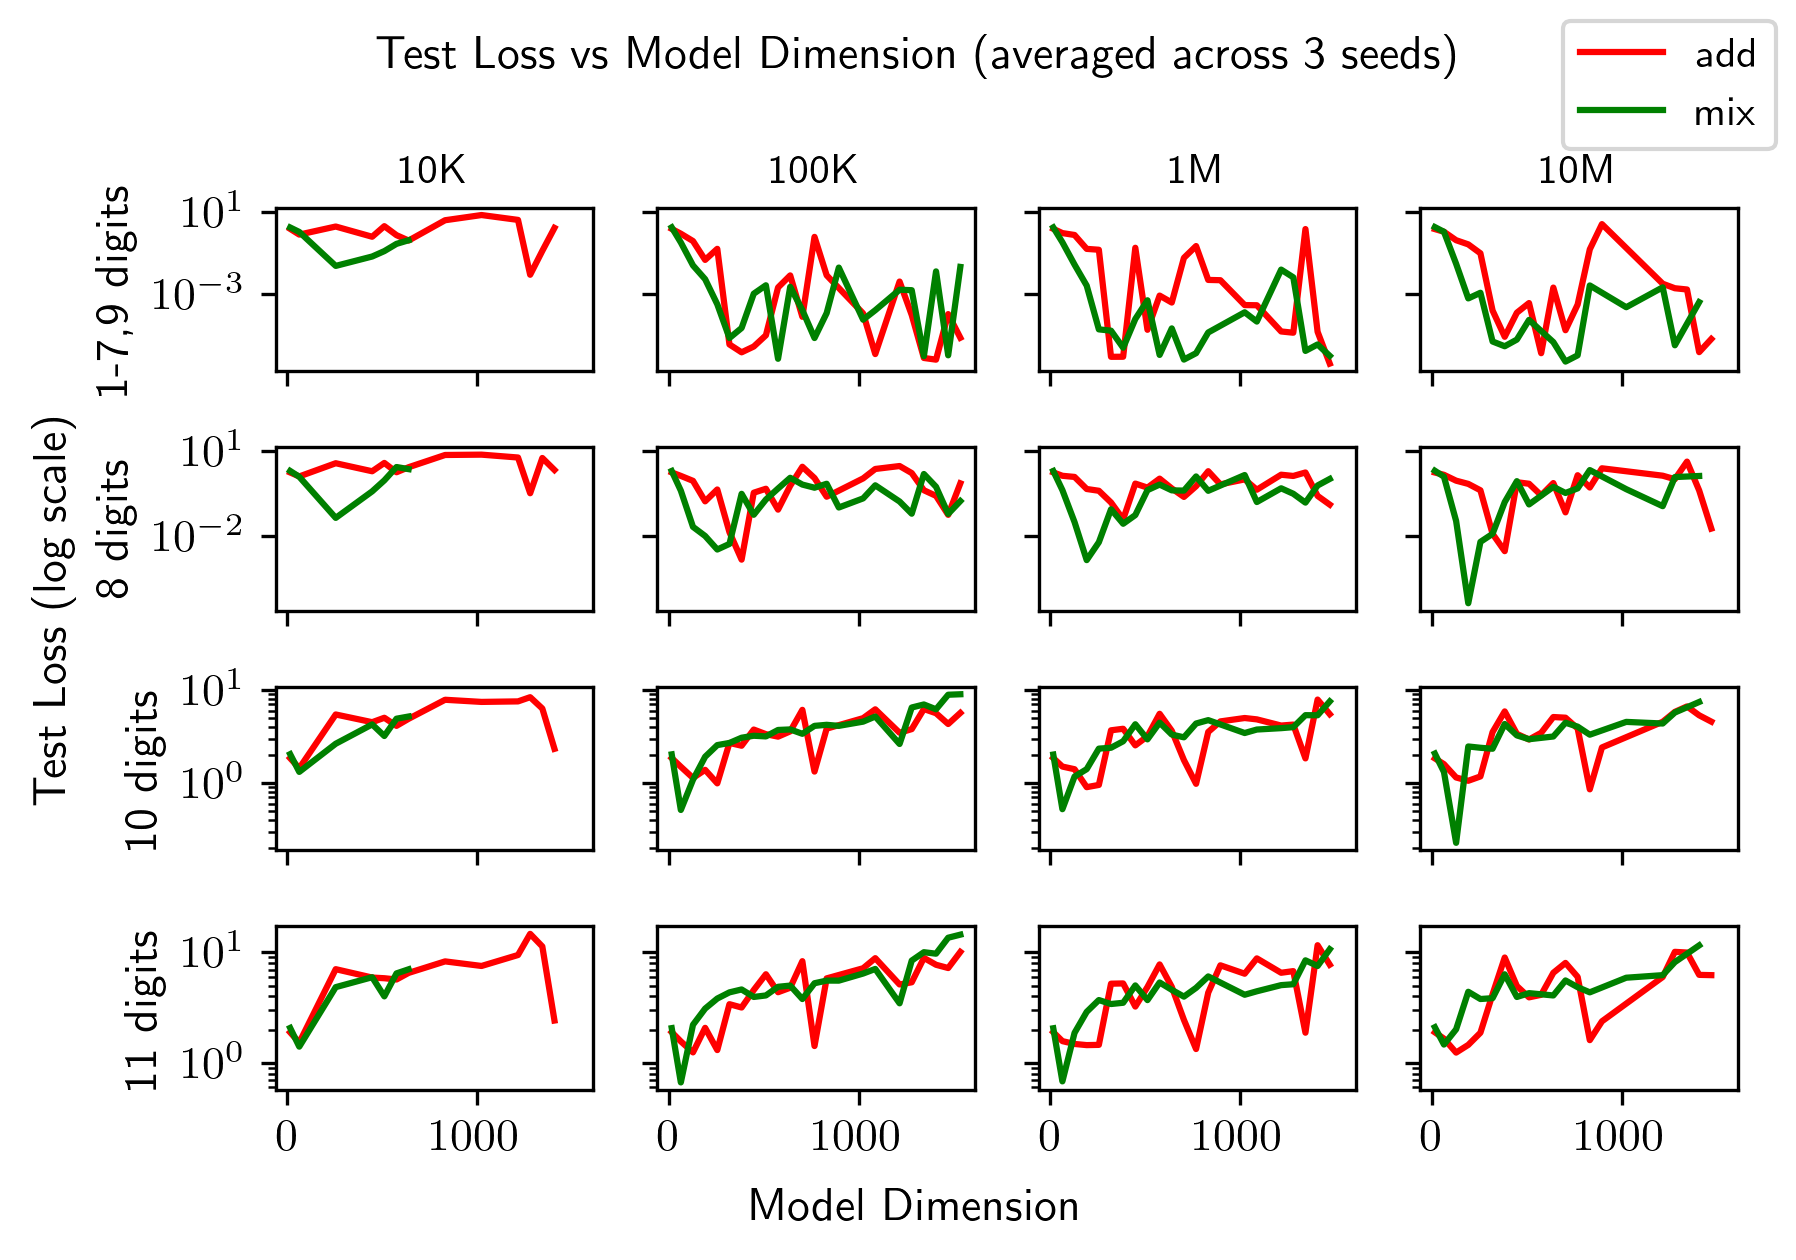
\includegraphics[width=\textwidth]{fig/exp_27_val_loss_vs_n_embd.png}
    \caption{TODO fix placeholder + caption, main idea: mix task training sometimes improves OOD loss, effect is especially pronounced for smaller models and smaller dataset sizes, but no clear effect in mid- and large models (over lengths evaluated).}
    \label{fig:exp_27_val_loss_vs_n_embd}
\end{figure}


\TODO{PLOT ID vs OOD losses to see if subtasks help overfitting. in some cases yes, can see a pareto improvement in OOD loss with no ID loss increase }
\label{fig:subtask_overfitting}

\subsection{Smaller Models Benefit More from Sub-Tasks}
Discuss how smaller models have lower OOD losses compared to larger models (no significant difference). Top difference

\TODO{PLOT 64 dim model across data sizes, add vs mix performance bar plots}
\label{fig:64_dim_performance}


\subsection{Sub-Task Difficulty and Learning Order}
Analysis of difficulty of subtasks and order in which they are learned. Also emphasize how some subtasks are unstable: could get 0 vs high accuracy after same number of training iterations depending on seed. Also look at learning order, some subtasks need to be learned first to help with others, that learning order is more or less consistent across different runs, as investigated using a similar method to \cite{lee_what_2022}.

\TODO{PLOT subtask difficulty across model sizes violin plots}
\label{fig:subtask_difficulty}

\TODO{PLOT subtask learning order over training runs, some subtasks need to be learned first to help with others}
\label{fig:subtask_order}
